\item {\bf Neural Networks: Fashion-MNIST image classification}

In this problem, you will implement a simple neural network
to classify grayscale images of clothings (10 labels: T-shirts, Trouser, Pullover, Dress, Coat, Sandal, Shirt, Sneaker, Bag, Ankel boot) from
the Fashion-MNIST dataset\footnote{\url{https://github.com/zalandoresearch/fashion-mnist}}
\footnote{This dataset is newly introduced from this cohort, which replaces MNIST, which is considered to be too easy nowadays.}
\footnote{The original Fashion-MNIST dataset is convered to the format for PS4 using this code \url{https://github.com/insop/Fashion-MNIST-csv}}.
This is a drop-in dataset replacement for MNIST\footnote{\url{https://en.wikipedia.org/wiki/MNIST_database}}.
The dataset contains 60,000 training images and
10,000 testing images of clothing types, 0 - 9. Each image is
28$\times$28 pixels in size, and is generally represented as a flat
vector of 784 numbers. It also includes labels for each example, a number
indicating the actual clothing types (0 - 9) that image. A sample of
a few such images are shown below.

\begin{center}
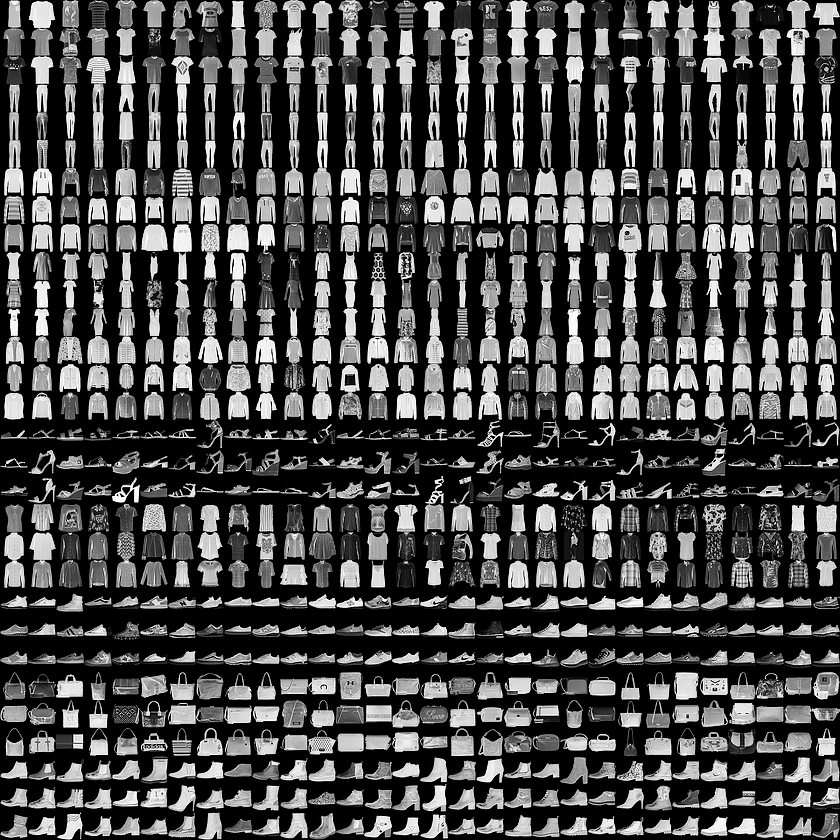
\includegraphics[scale=0.5]{02-mnist/fashion-mnist-sprite}
\end{center}


The data and starter code for this problem can be found in

\begin{itemize}
\item |src-mnist/submission.py|
\item |src-mnist/images_train.csv| (unzip |Archive.zip| to access this file)
\item |src-mnist/labels_train.csv| (unzip |Archive.zip| to access this file)
\item |src-mnist/images_test.csv| (unzip |Archive.zip| to access this file)
\item |src-mnist/labels_test.csv| (unzip |Archive.zip| to access this file)
\end{itemize}

The starter code splits the set
of 60,000 training images and labels into a set of 50,000 examples as
the training set, and 10,000 examples for dev set.

To start, you will implement a neural network with a single hidden layer
and cross entropy loss, and train it with the provided data set. Use the
sigmoid function as activation for the hidden layer, and softmax function
for the output layer. Recall that for a single example $(x, y)$, the cross
entropy loss is:
$$CE(y, \hat{y}) = - \sum_{k=1}^K y_k \log \hat{y_k},$$
where $\hat{y} \in \mathbb{R}^{K}$ is the vector of softmax outputs
from the model for the training example $x$,
and $y \in \mathbb{R}^{K}$ is the ground-truth vector for the training example
$x$ such that $y = [0,...,0,1,0,...,0]^\top$ contains a single 1 at the
position of the correct class (also called a ``one-hot'' representation).

For $\nexp$ training examples, we average the cross entropy loss over the $\nexp$ examples.
  \begin{equation*}
  J(W^{[1]},W^{[2]},b^{[1]},b^{[2]}) = \frac{1}{\nexp}\sum_{i=1}^\nexp CE(y^{(i)}, \hat{y}^{(i)}) = - \frac{1}{\nexp}\sum_{i=1}^\nexp \sum_{k=1}^K y_k^{(i)} \log \hat{y}_k^{(i)}.
  \end{equation*}
The starter code already converts labels into one hot representations for you.

Instead of batch gradient descent or stochastic gradient descent, the common practice
is to use mini-batch gradient descent for deep learning tasks. In this case, the
cost function is defined as follows:

  \begin{equation*}
  J_{MB} = \frac{1}{B}\sum_{i=1}^{B}CE(y^{(i)}, \hat{y}^{(i)})
  \end{equation*}
where $B$ is the batch size, i.e. the number of training example in each mini-batch. 

\begin{enumerate}
  \item \points{2a} 

Implement both forward-propagation and back-propagation for the above loss function.
More specifically you will implement the |softmax|, |sigmoid|, |get_initial_params|, |forward_prop|, 
|backward_prop|, and |gradient_descent_epoch| functions inside |src-mnist/submission.py|.

Initialize the weights of the network by sampling values from a standard normal
distribution. Initialize the bias/intercept term to 0.
Set the number of hidden units to be 300, and learning rate to be 0.4. Set $B = 1,000$
(mini batch size). This means that we train with 1,000 examples in each iteration.
Therefore, for each epoch, we need 50 iterations to cover the entire training data.
The images are pre-shuffled. So you don't need to randomly sample the data, and can
just create mini-batches sequentially.

Use autograder test case |2aii-6-basic| to train the model with mini-batch gradient descent
as described above. Before running this test case, edit line 186 of |src-mnist/grader.py| to state |skip = False| (model plotting/training is disabled by default to run the auotgrader faster). This will run the training for 30 epochs. At the end of each epoch, it will calculate
the value of loss function averaged over the entire training set.  It will then plot the average loss (y-axis) against the number of epochs (x-axis). In the same image, it will also plot the value of the loss function averaged over the dev set, and against the number of epochs.

This will also plot the accuracy (on y-axis) over the training set,
measured as the fraction of correctly classified examples, versus the number of epochs
(x-axis). In the same image, it will plot the accuracy over the dev set versus number of epochs.

\textbf{Hint:} Be sure to vectorize your code as much as possible! Training can be
very slow otherwise.

\clearpage\newpage

You plots should look similar to the following (You are not required to submit any plots.  These are for your own verification.):

\begin{figure}[H]
    \centering
    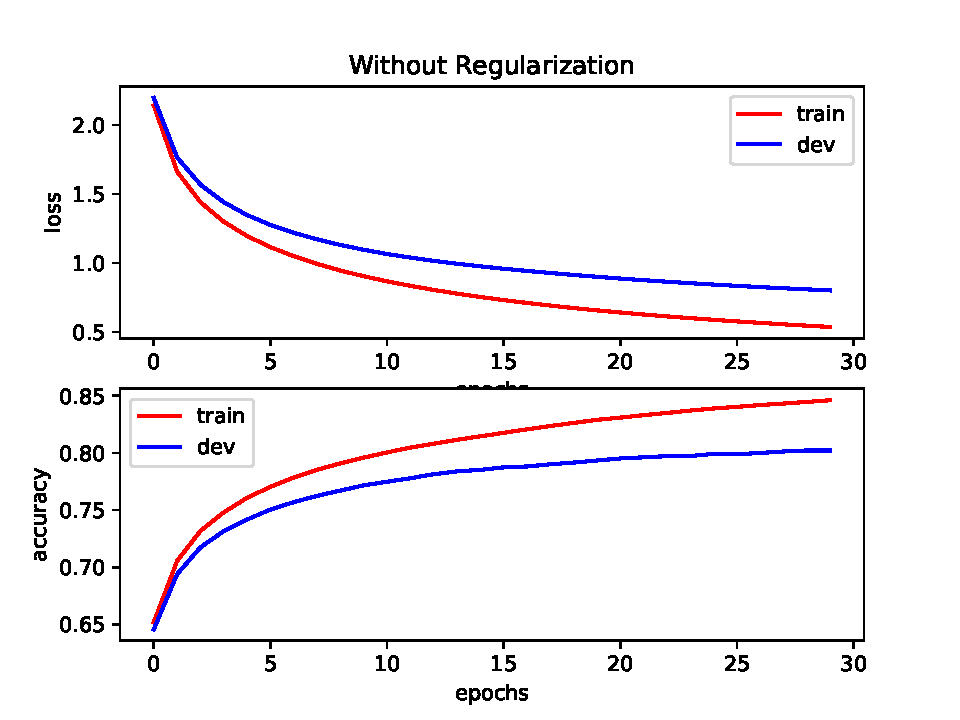
\includegraphics[scale=0.75]{02-mnist/baseline.pdf}
\end{figure}


  \item \points{2b} Now add a regularization term to your cross entropy loss by implementing |backward_prop_regularized()|.
The loss function will become \begin{equation*}
  J_{MB} = \left(\frac{1}{B}\sum_{i=1}^{B}CE(y^{(i)}, \hat{y}^{(i)})\right) + \frac{1}{2} \lambda \left(\vert \vert W^{[1]}\vert \vert ^2 + \vert \vert W^{[2]}\vert \vert ^2 \right)
  \end{equation*}

Autograder test case |2b-2-basic| will perform the same as |2aii-6-basic| (described earlier), except that it utilizes your new regularized backprop function.  Before running this test case, edit line 285 of |src-mnist/grader.py| to state |skip = False| (model plotting/training is disabled by default to run the auotgrader faster).  It will also plot the same
figures as part (a). Note that it does NOT include the regularization term to measure
the loss value for plotting (i.e., regularization should only be used for gradient calculation for
the purpose of training).

\clearpage\newpage
After creating the plots from the previous part, they should look similar to the following (You are not required to submit any plots.  These are for your own verification.):

\begin{figure}[H]
    \centering
    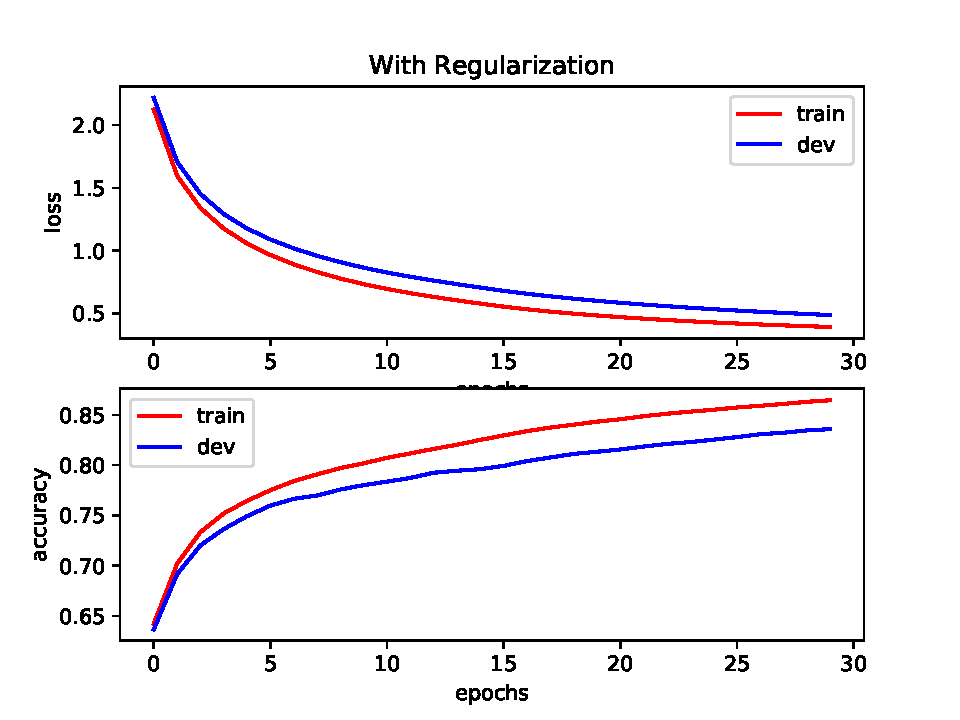
\includegraphics[scale=0.75]{02-mnist/regularized.pdf}
\end{figure}


  \item \points{2c}
All this while the test cases have avoided the test data completely. Now that
you have convinced yourself that the model is working as expected (i.e, the
observations you made in the previous part matches what you learnt in class
about regularization), it is finally time to measure the model performance on
the test set. Once we measure the test set performance, we report it (whatever
value it may be), and NOT go back and refine the model any further.

Autograder test case |2c-1-basic| will train your model and then evaluate its performance on the test data for both the regularized and non-regularized training strategies.  Before running this test case, edit line 361 of |src-mnist/grader.py| to state |skip = False| (model plotting/training is disabled by default to run the auotgrader faster).

You should have accuracy close to 0.7855 without regularization, and 0.819 with regularization.

Note: Even if you do not have precisely these numbers, you should observe better test accuracy with regularization than without.

Fashion-MNIST is challenging dataset compared to MNIST. With the similar hyperparameters, the accuracy of regularized model was 0.96 for MNIST dataset. Once you finished the assignment with given network specification, we encourage you to improve the accuracy by modifying the neural network model on your environment, such as adding more hidden layers, changing the hidden layer size, or using a different initialization. Once you do, please share your accuracy and model on
the slack PS4 channel!

 \end{enumerate}

